
I2C là một chuẩn được phát triển bởi Philips. Nó là một giao thức 2 dây chậm với tốc độ có thể lên đến 400 kHz. Nó được sử dụng rộng rãi trong hệ thống nhúng. Một số thiết bị sử dụng biến thể không đạt được yêu cầu của I2C nên có thể được gọi bằng tên khác như TWI hoặc IIC.

SMBus (System Management Bus) dựa trên giao thức I2C được sử dụng rộng rãi trong hệ thống máy tính. Rất nhiều thiết bị I2C có thể hoạt động trên SMBus như I2C EEPROMs và một số chip theo dõi phần cứng.

Trong một bus I2C, có thể có một hay nhiều master chip được kết nối tới một hay nhiều slave chip.


\begin{figure}[H]
	\centering
	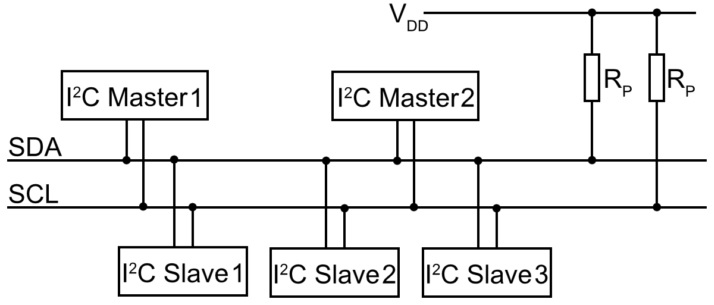
\includegraphics[width=0.6\textwidth]{images/I2C-Bus-Layout.jpg}
	\caption{I2C bus}
\end{figure}


Master chip là thiết bị kết nối tới slave. Trong nhân linux, master chip được gọi là một adapter hoặc bus. Các trình điều khiển của adapter nằm trong thư mục con drivers/i2c/busses.

Một algorithm chứa mã có thể sử dụng để cài đặt nhiều loại I2C adapter. Mỗi adapter driver có thể phụ thuộc vào một algorithm driver trong thư mục con drivers/i2c/algos hoặc chứa mã cho riêng nó.

Một slave chip là nút thực hiện giao tiếp khi có yêu cầu của master. trong Linux, nó được gọi là client. Client driver được lưu trong thư mục nào phụ thuộc vào các chức năng mà nó cung cấp, ví dụ như trong drivers/media/gpio cho thiết bị mở rộng GPIO.
